\documentclass[conference]{IEEEtran}
\makeatletter
\def\ps@headings{}
\def\@oddhead{\mbox{}\scriptsize\rightmark \hfil \thepage}%
\def\@evenhead{\scriptsize\thepage \hfil \leftmark\mbox{}}%
\def\@oddfoot{}
\def\@evenfoot{}
\makeatother
\pagestyle{headings}
\pagestyle{empty}
\usepackage{amsmath}
\usepackage{array}
\newcolumntype{P}[1]{>{\centering\arraybackslash}p{#1}}

\hyphenation{op-tical net-works semi-conduc-tor}


\usepackage{subfigure}

\usepackage{algorithmic}
\usepackage[ruled,vlined]{algorithm2e}

\ifCLASSINFOpdf
  \usepackage[pdftex]{graphicx}
  \graphicspath{ {./images/} }
  % declare the path(s) where your graphic files are
  % \graphicspath{{../pdf/}{../jpeg/}}
  % and their extensions so you won't have to specify these with
  % every instance of \includegraphics
  % \DeclareGraphicsExtensions{.pdf,.jpeg,.png}
\else
  % or other class option (dvipsone, dvipdf, if not using dvips). graphicx
  % will default to the driver specified in the system graphics.cfg if no
  % driver is specified.
  % \usepackage[dvips]{graphicx}
  % declare the path(s) where your graphic files are
  % \graphicspath{{../eps/}}
  % and their extensions so you won't have to specify these with
  % every instance of \includegraphics
  % \DeclareGraphicsExtensions{.eps}
\fi
% graphicx was written by David Carlisle and Sebastian Rahtz. It is
% required if you want graphics, photos, etc. graphicx.sty is already
% installed on most LaTeX systems. The latest version and documentation can
% be obtained at:
% http://www.ctan.org/tex-archive/macros/latex/required/graphics/
% Another good source of documentation is "Using Imported Graphics in
% LaTeX2e" by Keith Reckdahl which can be found as epslatex.ps or
% epslatex.pdf at: http://www.ctan.org/tex-archive/info/
%
% latex, and pdflatex in dvi mode, support graphics in encapsulated
% postscript (.eps) format. pdflatex in pdf mode supports graphics
% in .pdf, .jpeg, .png and .mps (metapost) formats. Users should ensure
% that all non-photo figures use a vector format (.eps, .pdf, .mps) and
% not a bitmapped formats (.jpeg, .png). IEEE frowns on bitmapped formats
% which can result in "jaggedy"/blurry rendering of lines and letters as
% well as large increases in file sizes.
%
% You can find documentation about the pdfTeX application at:
% http://www.tug.org/applications/pdftex

\begin{document}
\title{Better Approach to Geofence Detection}

% Author names 
% note positions of commas and nonbreaking spaces ( ~ ) LaTeX will not break
% a structure at a ~ so this keeps an author's name from being broken across
% two lines.
% use \thanks{} to gain access to the first footnote area
% a separate \thanks must be used for each paragraph as LaTeX2e's \thanks
% was not built to handle multiple paragraphs
\author{
Andrea Sghedoni MATR.0000736038\IEEEauthorrefmark{1},
\\
\IEEEauthorblockA{\IEEEauthorrefmark{1} DISI, University of Bologna, Italy \\
 \\
Email: andrea.sghedoni4@studio.unibo.it}}




% make the title area
\maketitle

% The Abstract
\begin{abstract}
My Location Alert is a smartphone application developed for the Android operating system.
The app allows you to create fences, selecting a center and a range, and capture all ENTER/EXIT events.
Whenever you experience any of these events, it is automatically sent an alert SMS to a mobile (previously selected).
The main goal of the project, however, is to compare the battery consumption of two strategies/services for location monitoring in time.
The first strategy is based on the simple polling strategy, while the second adopt a smarter auto-adaptive approach to avoid an excessive battery consumption, which would make the app unusable.

\end{abstract}



\section{Introduction}
The geofencing approach means taking monitored geographical area and giving awareness to the device of the EXIT/ENTER/REMAIN events in one place.
Location Services is one of the most important cause of battery discharge in smartphones.
If these services must to be continuous in time (with active jobs in background), it is likely the user to view a major deterioration of the battery.
In recent years, Google is committed to the improvement of these activities, especially to reach an optimum point between precision and consumption.
Please note that the location can be basically made from two mechanisms:
the first concerns the use of the GPS sensor and has an important consumption of battery in the phone, while the second concerns the use of the network, even if in this precision is less, in comparison to the use of GPS sensor.
Most of geofence mechanisms adopt a polling strategy. which controls the position at constant intervals (~ 5 sec, ~ 10 sec, ...). This method, if it is merged with the use of GPS, drains battery in few hours. Considering also that the user, of course, does not use the smartphone only for geofencing, but we must also take account of all the other apps that users install, use and need.
The main goal project is to implement an intelligent mechanism for which the position is monitored frequently and with the GPS only if you are close to a fence, while controlling the position less frequently (and via network, to a lower consumption) as that the device moves away from the user-selected geofences.
The approach relies on an auto-adaptive mechanism, where the algorithm tries to use certain resources only when necessary, details will still in Section III.
The project was developed as part of Mobile Systems exam at Alma mater Studiorum, Bologna.
The main use case of My Location Alert app is automatically alert a phone number (via SMS) of entry/exit events from a specific geographic region. 

\section{Related works}
Fornisci una breve rassegna di articoli di ricerca, software, prototipi o tecnologie che sono collegate in qualche modo al problema affrontato nel progetto. Tutti i lavori devono essere referenziati ed inseriti nella Bibliografia.

\section{Architecture}
Basically, the app is composed with the two traditional components, such as frontend and backend.
The first component is represented by the graphic interface with which the user interacts, such as maps, registration forms fence etc.
The most interesting part is the back-end, which is composed of: Entity, SQLiteManager, Controller, Services.

\begin{figure}[h]
\centering
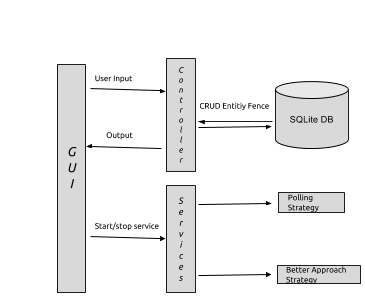
\includegraphics[scale=0.6]{architecture}
\caption{Architecture}
\end{figure}

\textit{Entity} map a fence in a java object that contains all the information needed to manage it, such as to address, latitude, longitude, range, state, activation, event to detect.
\\\textit{SQLiteManager} manages the database, provides methods for CRUD(create, read, update, delete) data of the fence.
This allows you to record your preferences.
The DB is composed of a single table, in which each entry corresponds to a fence, registered by users and each column map an attribute of the Java class Fence.
\\The \textit{Controller} is an object that implements Singleton pattern, only one instance of that class is created and accessed.
It exposes data and methods that should be available and accessed from anywhere in the project.
Mainly, it provides the current user fence list and acts as interface to the SQLite DB, providing functions that implement CRUD verbs.
\\\textit{Services} implement the monitoring and detection strategies of registred fences, which run in the background even when the app is not open.
Only one of the two services can be active at a given time.
The performance differences between the two services implemented is the true heart of the project, you will see in the results that the polling startegy produces a battery consumption exaggerated relative to the other auto-adaptive strategy.

\section{Implementation}
Android Studio is the official IDE for Android, where you can test code on different device emulators and monitor log.
The development of a native Android app requires the use of object-oriented language JAVA.
With regard to the persistence of the information (basically the Fence objects with their attributes) entered by the user it has been necessary to create and maintain a DataBase SQLite.
We have used various services of google map api Android, from the representation of the map (markers, fence circles) to use of location services (location update requests).
In addition, the Geocoding service allows the user to select the center of fence, with an address directly and not with latitude and longitude.
Git is used as a version control system, very important for step-by-step development and progress monitoring.\\
Location monitoring and fence events detection are the most important jobs that she must implement.\\
The first strategy acts polling, which get GPS position every 5 seconds (costant updates). LocationRequest, in this method, use $PRIORITY\_HIGH\_ACCURACY$ like priority parameter.\\
The second strategy is a smart approach, which goal is a better low battery consumption.
This method uses the most expensive in terms of energy resources, such as a GPS sensor, only when absolutely necessary. This means that if the device is very close to the fences will access the location more frequently, 
looking for accurate precision. Conversely if your smartphone is away from fences, recorded by the user, the position is monitored less frequently and not with the use of GPS sensor, but taking it from the network.\\
The approach is self-adaptive and dynamically change the frequency and precision of the location updates.
The algorithm is based on 3 balaced parameters: distance (between fence and current location), device speed and direction.
Each of these parameters are mapped on a scale from 0 to 5, and multiplied by a coefficient, the total of the three parameters approximate sum indicates the frequency and 
the accuracy of the position updates.
The most influential parameter is the distance from the fence (0.8), but also the direction and speed parameters can make change plan.

\begin{subequations}\label{grp}
  \begin{align}
    \alpha&=0.8\label{second}\\
    \beta&=0.1\label{third}\\
    \gamma&=0.1\label{fourth}
  \end{align}
\end{subequations}

fdddddddddddddd

\begin{equation}[h]
\boxed{f_i = \alpha f(distance) + \beta f(direction) + \gamma f(speed)}
\end{equation}

\begin{table}[h]
  \centering
    \begin{tabular}{|P{2.5cm}|P{2.5cm}|}
    \hline
    Distance(meters) & f(distance)\\ \hline
    $<$ 8000 & 5\\ \hline
    8000-30000 & 4\\ \hline
    30000-50000 & 3\\ \hline
    50000-100000 & 2\\ \hline
    100000-200000 & 1\\ \hline
    $>$ 200000 & 0\\ \hline
    \end{tabular}
  \newline\newline
  \caption{Distance evaluation}
\end{table}

\begin{table}
  \centering
    \begin{tabular}{|P{2.5cm}|P{2.5cm}|}
    \hline
    Speed(Km/h) & f(speed)\\ \hline
    $>$ 130 & 5\\ \hline
    130-100 & 4\\ \hline
    100-60 & 3\\ \hline
    60-20 & 2\\ \hline
    $<$ 20 & 1\\ \hline
   \end{tabular}
  \newline\newline
  \caption{Speed evaluation}
\end{table}

\begin{table}
  \centering
    \begin{tabular}{|P{2.5cm}|P{2.5cm}|}
    \hline
    Direction & f(direction)\\ \hline
    Yes & 5\\ \hline
    No & 0\\ \hline
    \end{tabular}
  \newline\newline
  \caption{Direction evaluation}
\end{table}


\begin{table}
  \centering
    \begin{tabular}{|P{1cm}|P{2cm}|P{5.5cm}|}
    \hline
    $f_i$ & Interval(second) & LocationRequest Precision \\ \hline
    5 & 5 &  \tiny$PRIORITY\_HIGH\_ACCURACY$ \\ \hline
    4 & 30 &  \tiny$PRIORITY\_BALANCED\_POWER\_ACCURACY$ \\ \hline
    3 & 60 &  \tiny$PRIORITY\_BALANCED\_POWER\_ACCURACY$ \\ \hline
    2 & 180 &  \tiny$PRIORITY\_LOW\_POWER$ \\ \hline
    1 & 300 &  \tiny$PRIORITY\_LOW\_POWER$ \\ \hline
    0 & 480 &  \tiny$PRIORITY\_LOW\_POWER$ \\ \hline
   \end{tabular}
  \newline\newline
  \caption{Evaluation strategies}
\end{table}
 
\section{Performance evaluation}
Illustra qui i risultati sperimentali (simulazioni o esperimenti) che catturano le prestazioni del sistema realizzato. Chiarisci quali sono gli indici di stima
e come sono calcolati. Inserisci un breve commento per ogni grafico.

\section{Conclusioni}
Conclusioni, possibili sviluppi futuri e limitazioni del progetto realizzato

%% Inserisci bibliografia dei lavori citati (consiglio l'utilizzo di bibtex)
\bibliographystyle{plain}
\begin{thebibliography}{15}

\bibitem{NomeRiferimento}
\newblock{Lista Autori} 
\newblock{Titolo Lavoro}
\newblock{\textit{Nome Rivista o Convegno}}, pagine, anno pubblicazione.

\end{thebibliography}
\end{document}
